\section{Simplification of the Navier-Stokes equation (21-25)}

\subsection{Simplification I: incompressible flows}
Incompressibility means that the density of a fluid particle (moving along its pathline) remains constant.

Incompressiblity is a very good approximation for most liquids, including water. In $\SI{1000}{m}$ depth the density of seawater is only $0.4\%$ larger that at the surface. For gas glows incompressiblity is also a good approximation as long as $|\vec{u}_\mathrm{gas}| \ll \mathrm{speed\ of\ sound}$. Compressibility becomes important when discussing e.g. sound waves.

\begin{align}
0 = \diff{\rho(\vec{r},t)}{t} &= \pdiff{\rho}{t}+\left(\vec{u}\cdot\vec{\nabla}\right)\rho\\
&= -\vec{\nabla}\left(\rho\vec{u}\right)+\left(\vec{u}\cdot\vec{\nabla}\right)\rho \\
&= -\left(\vec{u}\cdot\vec{\nabla}\right)\rho - \rho\left(\vec{\nabla}\cdot\vec{u}\right) + \left(\vec{u}\cdot\vec{\nabla}\right)\rho\\
&= -\rho\left(\vec{\nabla}\cdot\vec{u}\right)\\
&= -\rho\, \mathrm{div}\, \vec{u}
\end{align}
In the first line we used the material derivative. In the step to the second line we used continuity equation.

For incompressibility the divergence must be zero:
\begin{equation}
\vec{\nabla}\cdot\vec{u} = 0
\end{equation}

Navier-Stokes equation for incompressible flows:
\begin{equation}
\rho\left(\pdiff{\vec{u}}{t}+\left(\vec{u}\cdot\vec{\nabla}\right)\right)\vec{u} = f_\mathrm{ext}-\vec{\nabla}p+\mu\left(\vec{\nabla}\cdot\vec{\nabla}\right)\vec{u}
\end{equation}
\begin{framed}
Remark: It looks simple, but these nonlinear differential equations remain a formidable challenge to engineers, physicists and mathematicians.
\end{framed}
Equation of state in the simplest form with constant density:
\begin{equation}
p=p(\rho) \Rightarrow \rho=\rho_0=\mathrm{constant}
\end{equation}


\subsection{Simplification II: incompressible, ideal, stationary, irrotational flows}
We use the incompressibility result from earlier:
\begin{equation}
\vec{\nabla}\cdot\vec{u} = 0
\end{equation}

Ideal means no friction. To eliminate friction forces we set $\mu=0$.

Euler equation:
\begin{equation}
\rho_0\left(\pdiff{\vec{u}}{t}+\left(\vec{u}\cdot\vec{\nabla}\right)\vec{u}\right) = f_\mathrm{ext}-\vec{\nabla}p
\end{equation}

stationary:
\begin{align}
\vec{u}(\vec{r},t) &= \vec{u}(\vec{r})\\
\leadsto
\pdiff{\vec{u}}{t} &= 0
\end{align}
\begin{equation}
\rho_0\left(\vec{u}\cdot\vec{\nabla}\right)\vec{u} = f_\mathrm{ext}-\vec{\nabla}p
\end{equation}

no external forces: $f_\mathrm{ext}=0$
\begin{equation}
\rho_0\left(\vec{u}\cdot\vec{\nabla}\right)\vec{u} = -\vec{\nabla}p
\end{equation}

Assuming irrotational flow: $\vec{\nabla}\times\vec{u}=0$.
\begin{equation}
\vec{\nabla}\underbrace{\left(\frac{\rho_0}{2}\vec{u}^2+p\right)}_\mathrm{constant}=0
\end{equation}

Bernoulli's equation
\begin{align}
\frac{\rho_0}{2}\vec{u}^2+p &= \mathrm{constant}\\
\vec{\nabla}\cdot\vec{u} &= 0\\
\vec{\nabla}\times\vec{u} &= 0
\end{align}
Given all the assumptions, this set of equations is equivalent to the Navier-Stokes equation.

\begin{shaded}
I skipped page 23a and 23b. Should these be included here?
\end{shaded}


\subsection{Derivation of Bernoulli's equation}
The equation
\begin{equation}
\vec{\nabla}\left(\frac{\rho_0}{2}\vec{v}^2+p\right) = \rho_0\vec{v}\times\left(\vec{\nabla}\times\vec{v}\right)
\end{equation}
is (scalar) multiplied with $d\vec{s}\parallel\vec{v}$, where $d\vec{s}$ describes an increment of a specific streamline (here pathline since $\vec{v}(\vec{r},t) = \vec{v}(\vec{r})$).
\begin{equation}
d\vec{s}\cdot\left[\vec{v}\times\left(\vec{\nabla}\times\vec{v}\right)\right]=0
\end{equation}
Since $d\vec{s}\parallel\vec{v}$ it must be that $d\vec{s}\perp\vec{v}\times\left(\vec{\nabla}\times\vec{v}\right)$.

Subsequent path-integration along a streamline yields
\begin{align}
0 \require ...
\end{align}


\subsection{Example: Why does an airplane fly?}
\begin{figure}[!h]
    \centering
    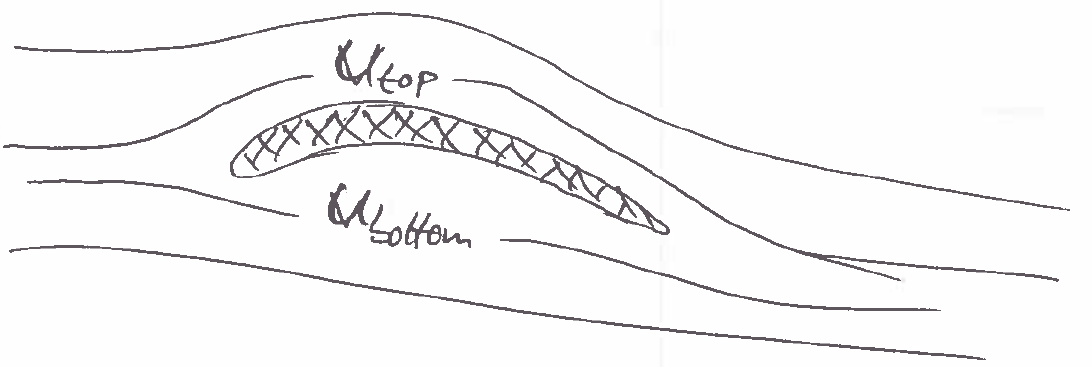
\includegraphics[width=.6\textwidth]{week2/airplane}
    \caption{}
    \label{fig:airplane}
\end{figure}
The wind speed difference between the top and bottom of the wing creates a pressure difference:
\begin{align}
u_\mathrm{top} &> u_\mathrm{bottom}\\
\leadsto
p_\mathrm{top} &< p_\mathrm{bottom}.
\end{align}
This results in a lifting force.